\chapter{Métodos}
\label{metodos}

Este capítulo describe la metodología empleada en el desarrollo del sistema de aprendizaje de idiomas, incluyendo la arquitectura del sistema, la implementación de los componentes, los algoritmos desarrollados y la metodología de evaluación.

\section{Arquitectura del Sistema}
\label{arquitectura-sistema}

El sistema se ha diseñado siguiendo una arquitectura modular y escalable que integra tecnologías de vanguardia en \gls{ia} y procesamiento de lenguaje natural. La arquitectura se divide en dos componentes principales: frontend y backend, comunicados a través de una \gls{api-rest}.

\begin{figure}[H]
	\centering
	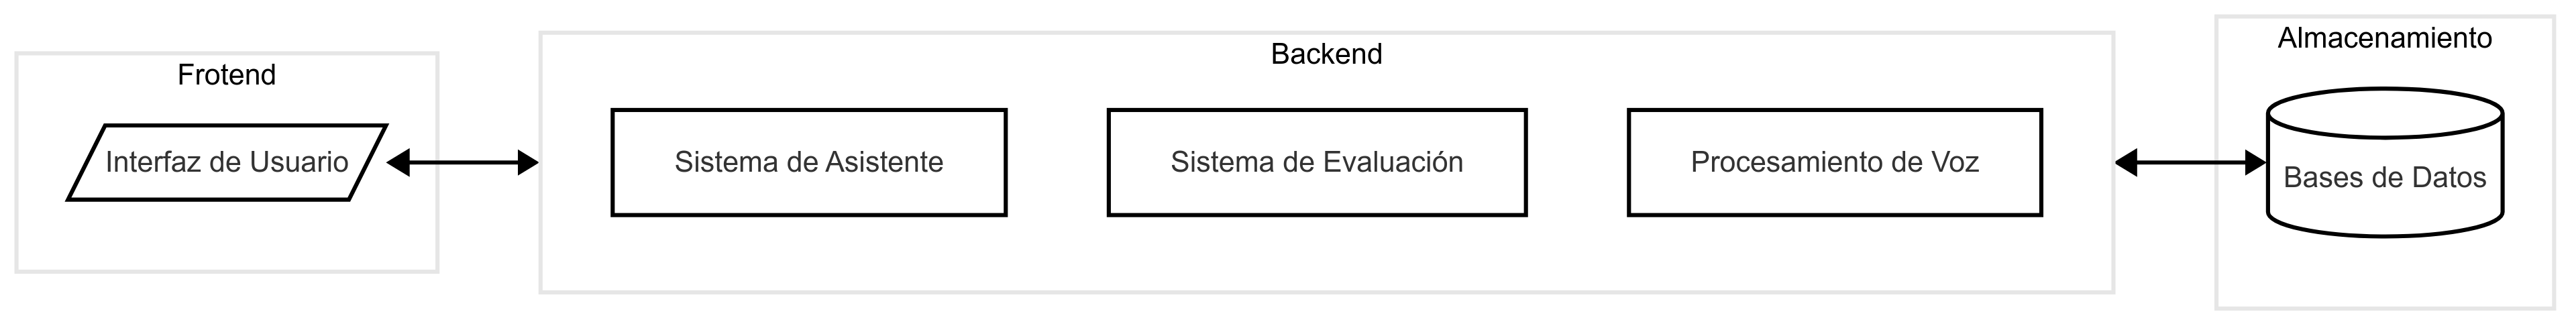
\includegraphics[width=0.8\textwidth]{figuras/system-overview.png}
	\caption{Arquitectura Simplificada del Sistema}
	\label{fig:arquitectura-sistema}
\end{figure}


\subsection{Frontend}
\label{frontend}

El frontend del sistema se implementa utilizando Next.js y está basado en el framework \gls{assistant-ui}, un proyecto \gls{open-source} que facilita la integración de interfaces de chat con LangGraph. Esta decisión arquitectónica permite una rápida implementación de funcionalidades de chat mientras mantiene la flexibilidad para personalizaciones específicas del dominio.

\begin{figure}[H]
	\centering
	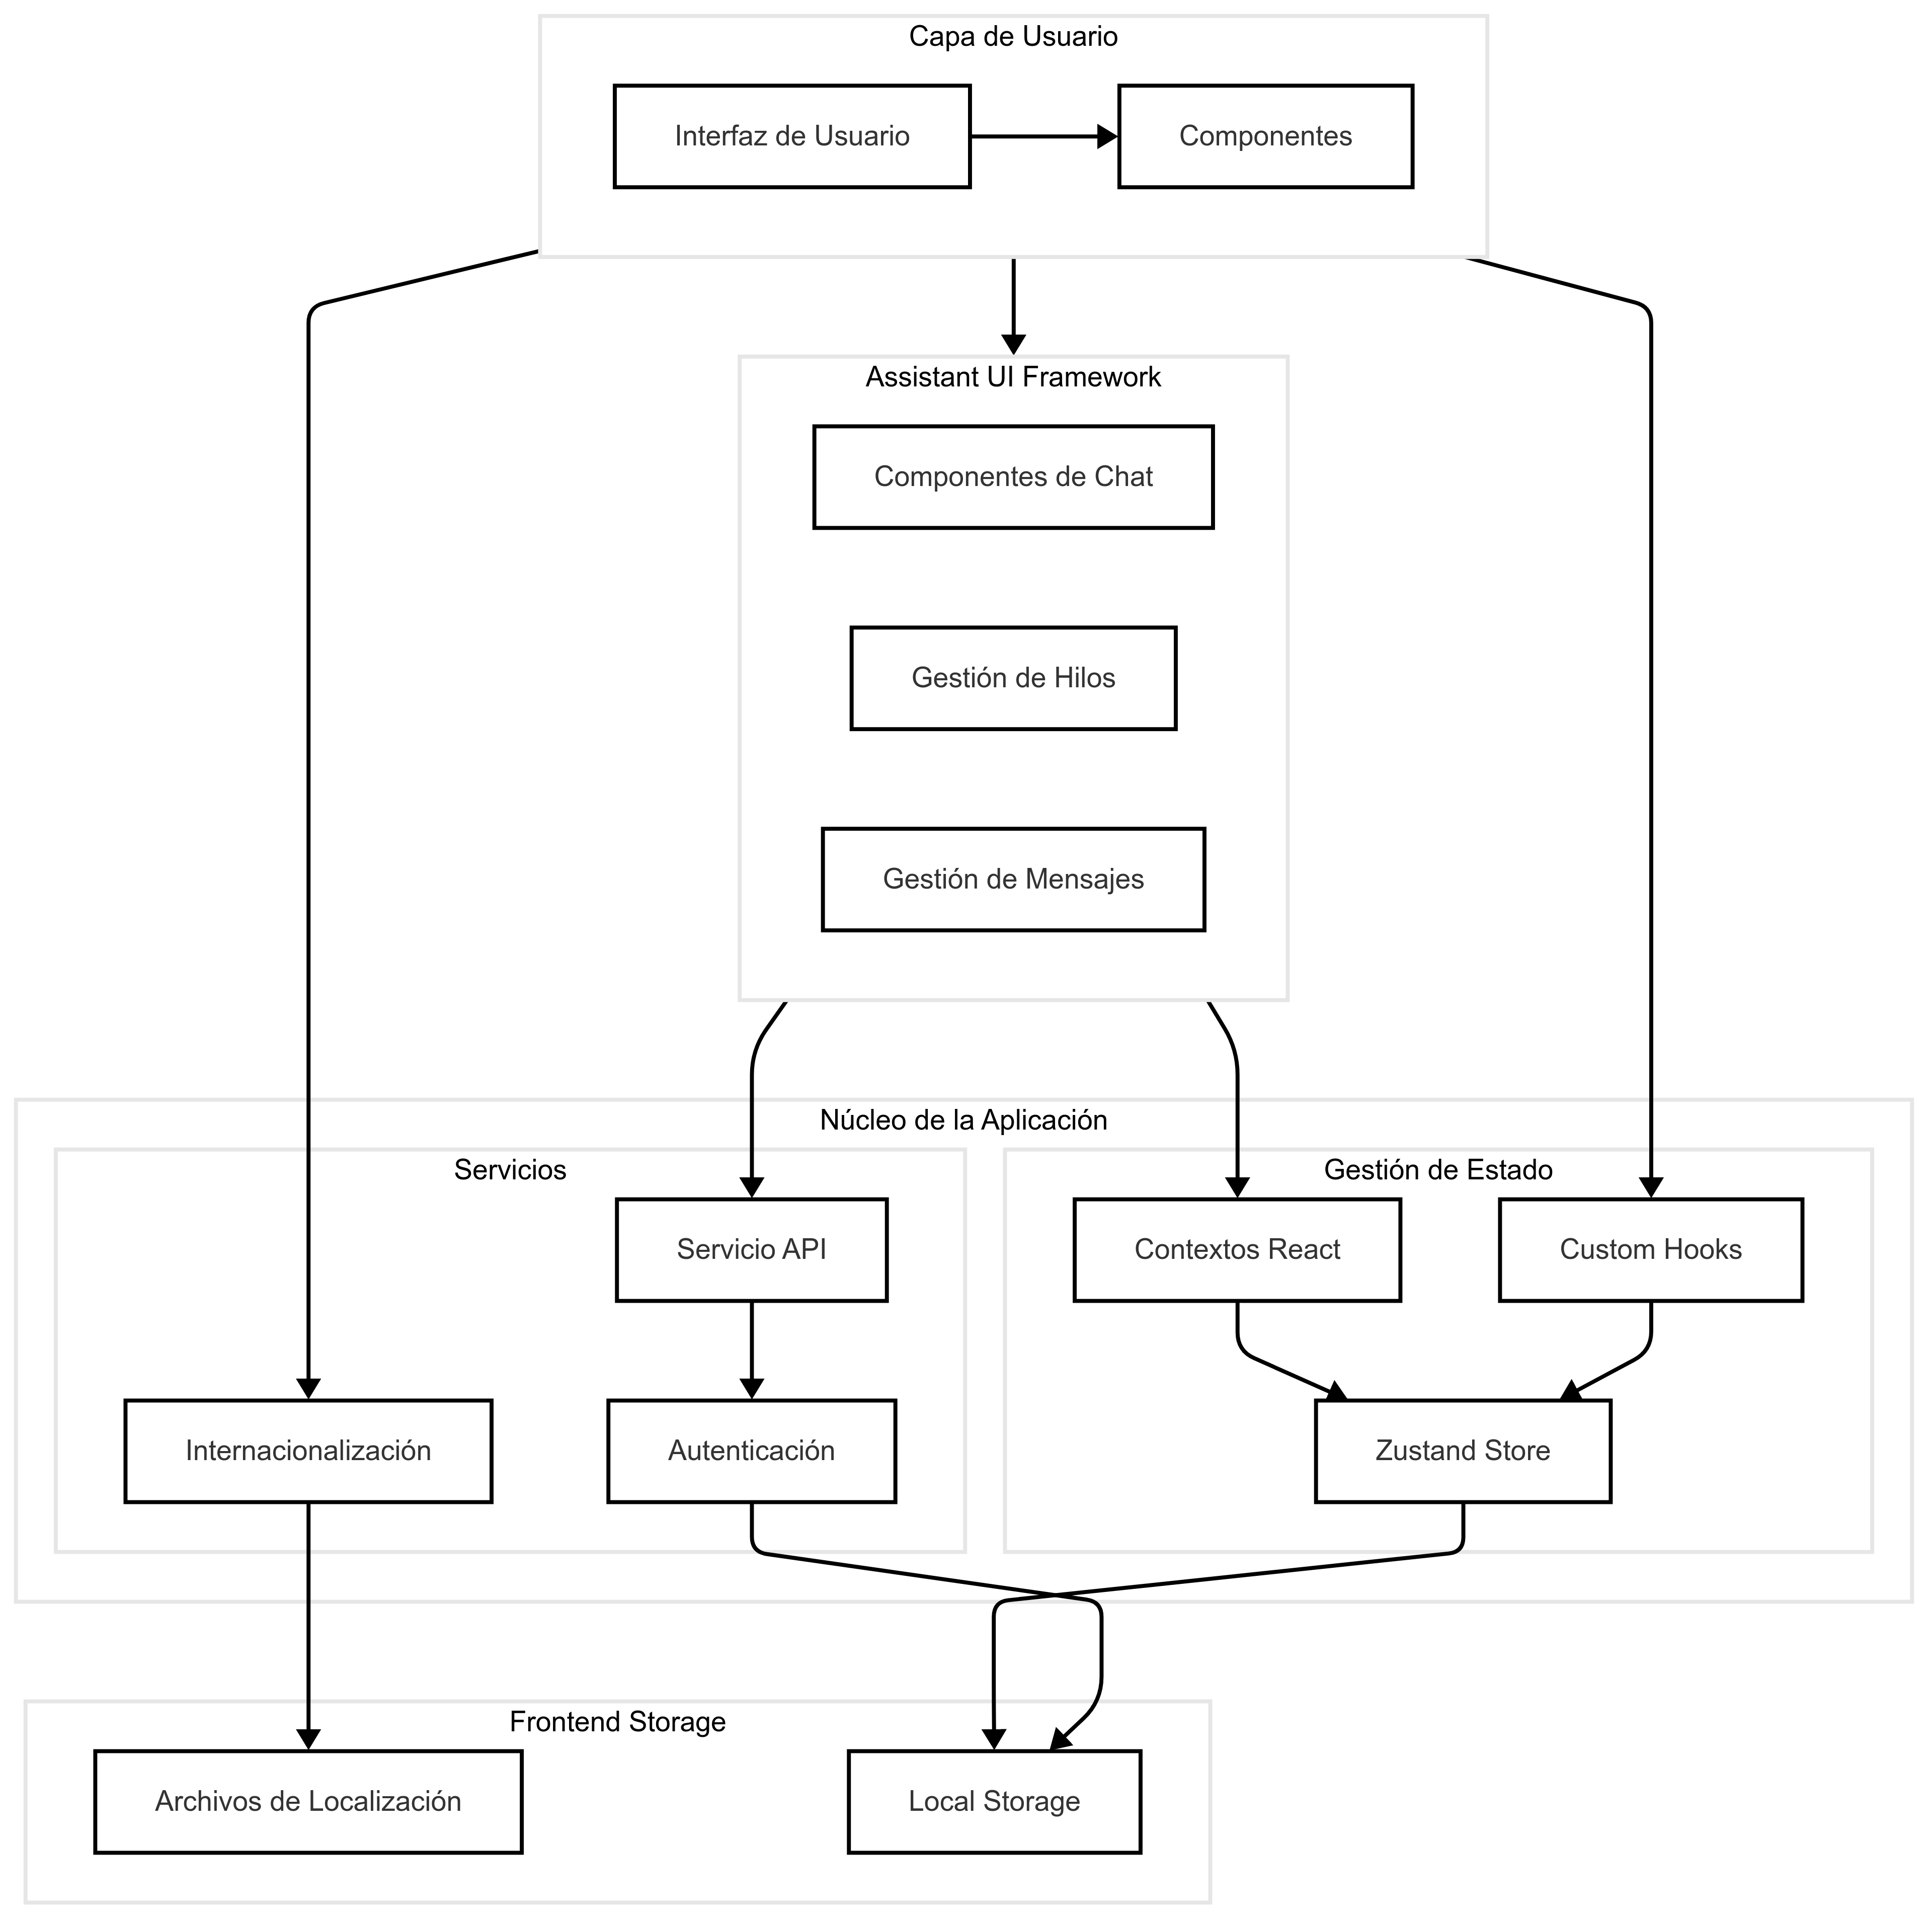
\includegraphics[width=0.8\textwidth]{figuras/frontend.png}
	\label{fig:arquitectura-frontend}
	\caption{Arquitectura del Frontend}
\end{figure}

\subsubsection{Assistant UI Framework}
\label{assistant-ui}

El sistema se construye sobre \gls{assistant-ui}, que proporciona:

\begin{itemize}
	\item \textbf{Componentes de Chat}:
	      \begin{itemize}
		      \item Interfaz de chat prediseñada y personalizable
		      \item Sistema de renderizado de mensajes
		      \item Gestión de entrada de usuario
	      \end{itemize}

	\item \textbf{Gestión de Hilos}:
	      \begin{itemize}
		      \item Sistema de hilos de conversación
		      \item Persistencia de contexto conversacional
		      \item Manejo de múltiples conversaciones
	      \end{itemize}

	\item \textbf{Gestión de Mensajes}:
	      \begin{itemize}
		      \item Sistema de cola de mensajes
		      \item Gestión de estados de mensajes
		      \item Manejo de respuestas asíncronas
	      \end{itemize}
\end{itemize}
\subsubsection{Arquitectura de Componentes}
La arquitectura del frontend se organiza en las siguientes capas:

\begin{itemize}
	\item \textbf{Capa de Usuario}:
	      \begin{itemize}
		      \item Implementación de páginas y rutas utilizando el sistema de enrutamiento de Next.js
		      \item Implementación de layouts y templates adaptables
		      \item Integración con el sistema de internacionalización
	      \end{itemize}

	\item \textbf{Núcleo de la Aplicación}:
	      \begin{itemize}
		      \item Gestión de estado utilizando Zustand para el manejo de datos de roleplay, progreso y reportes
		      \item Servicios para comunicación con el backend
		      \item Sistema de internacionalización con archivos de localización
	      \end{itemize}

	\item \textbf{Utilidades}:
	      \begin{itemize}
		      \item Funciones de validación y formateo
		      \item Manejadores de errores globales
		      \item Helpers para formateo y transformación de datos
		      \item Adaptadores para internacionalización
	      \end{itemize}
\end{itemize}

\subsubsection{Gestión de Estado}
\label{gestion-estado}

El sistema utiliza Zustand como solución de gestión de estado, proporcionando:

\begin{itemize}
	\item \textbf{Estado Global}:
	      \begin{itemize}
		      \item Gestión del estado del roleplay
		      \item Seguimiento del progreso del usuario
		      \item Almacenamiento de reportes de actividad
	      \end{itemize}

	\item \textbf{Persistencia}:
	      \begin{itemize}
		      \item Integración con localStorage para persistencia de datos
		      \item Sincronización de estado entre sesiones
		      \item Gestión de caché de datos
	      \end{itemize}
\end{itemize}

\subsubsection{Servicios de Comunicación}
\label{servicios-comunicacion}

La comunicación con el backend se gestiona a través de servicios especializados:

\begin{itemize}
	\item \textbf{API Service}:
	      \begin{itemize}
		      \item Implementación de cliente HTTP basado en Axios
		      \item Sistema de interceptores para manejo de errores
		      \item Caché de respuestas para optimización de rendimiento
	      \end{itemize}

	\item \textbf{Gestión de Autenticación}:
	      \begin{itemize}
		      \item Sistema de autenticación basado en tokens
		      \item Manejo de sesiones de usuario
		      \item Protección de rutas y recursos
	      \end{itemize}

	\item \textbf{Servicio de Internacionalización}:
	      \begin{itemize}
		      \item Gestión de traducciones y locales
		      \item Cambio dinámico de idioma
		      \item Formateo de fechas y números según la localización
	      \end{itemize}
\end{itemize}

\subsection{Backend}
\label{backend}

El backend del sistema se implementa utilizando FastAPI como framework principal, incorporando un sistema multi-agente basado en LangGraph para la gestión de la lógica de aprendizaje. La arquitectura se organiza en capas claramente definidas que gestionan diferentes aspectos del sistema.

\begin{figure}[H]
	\centering
	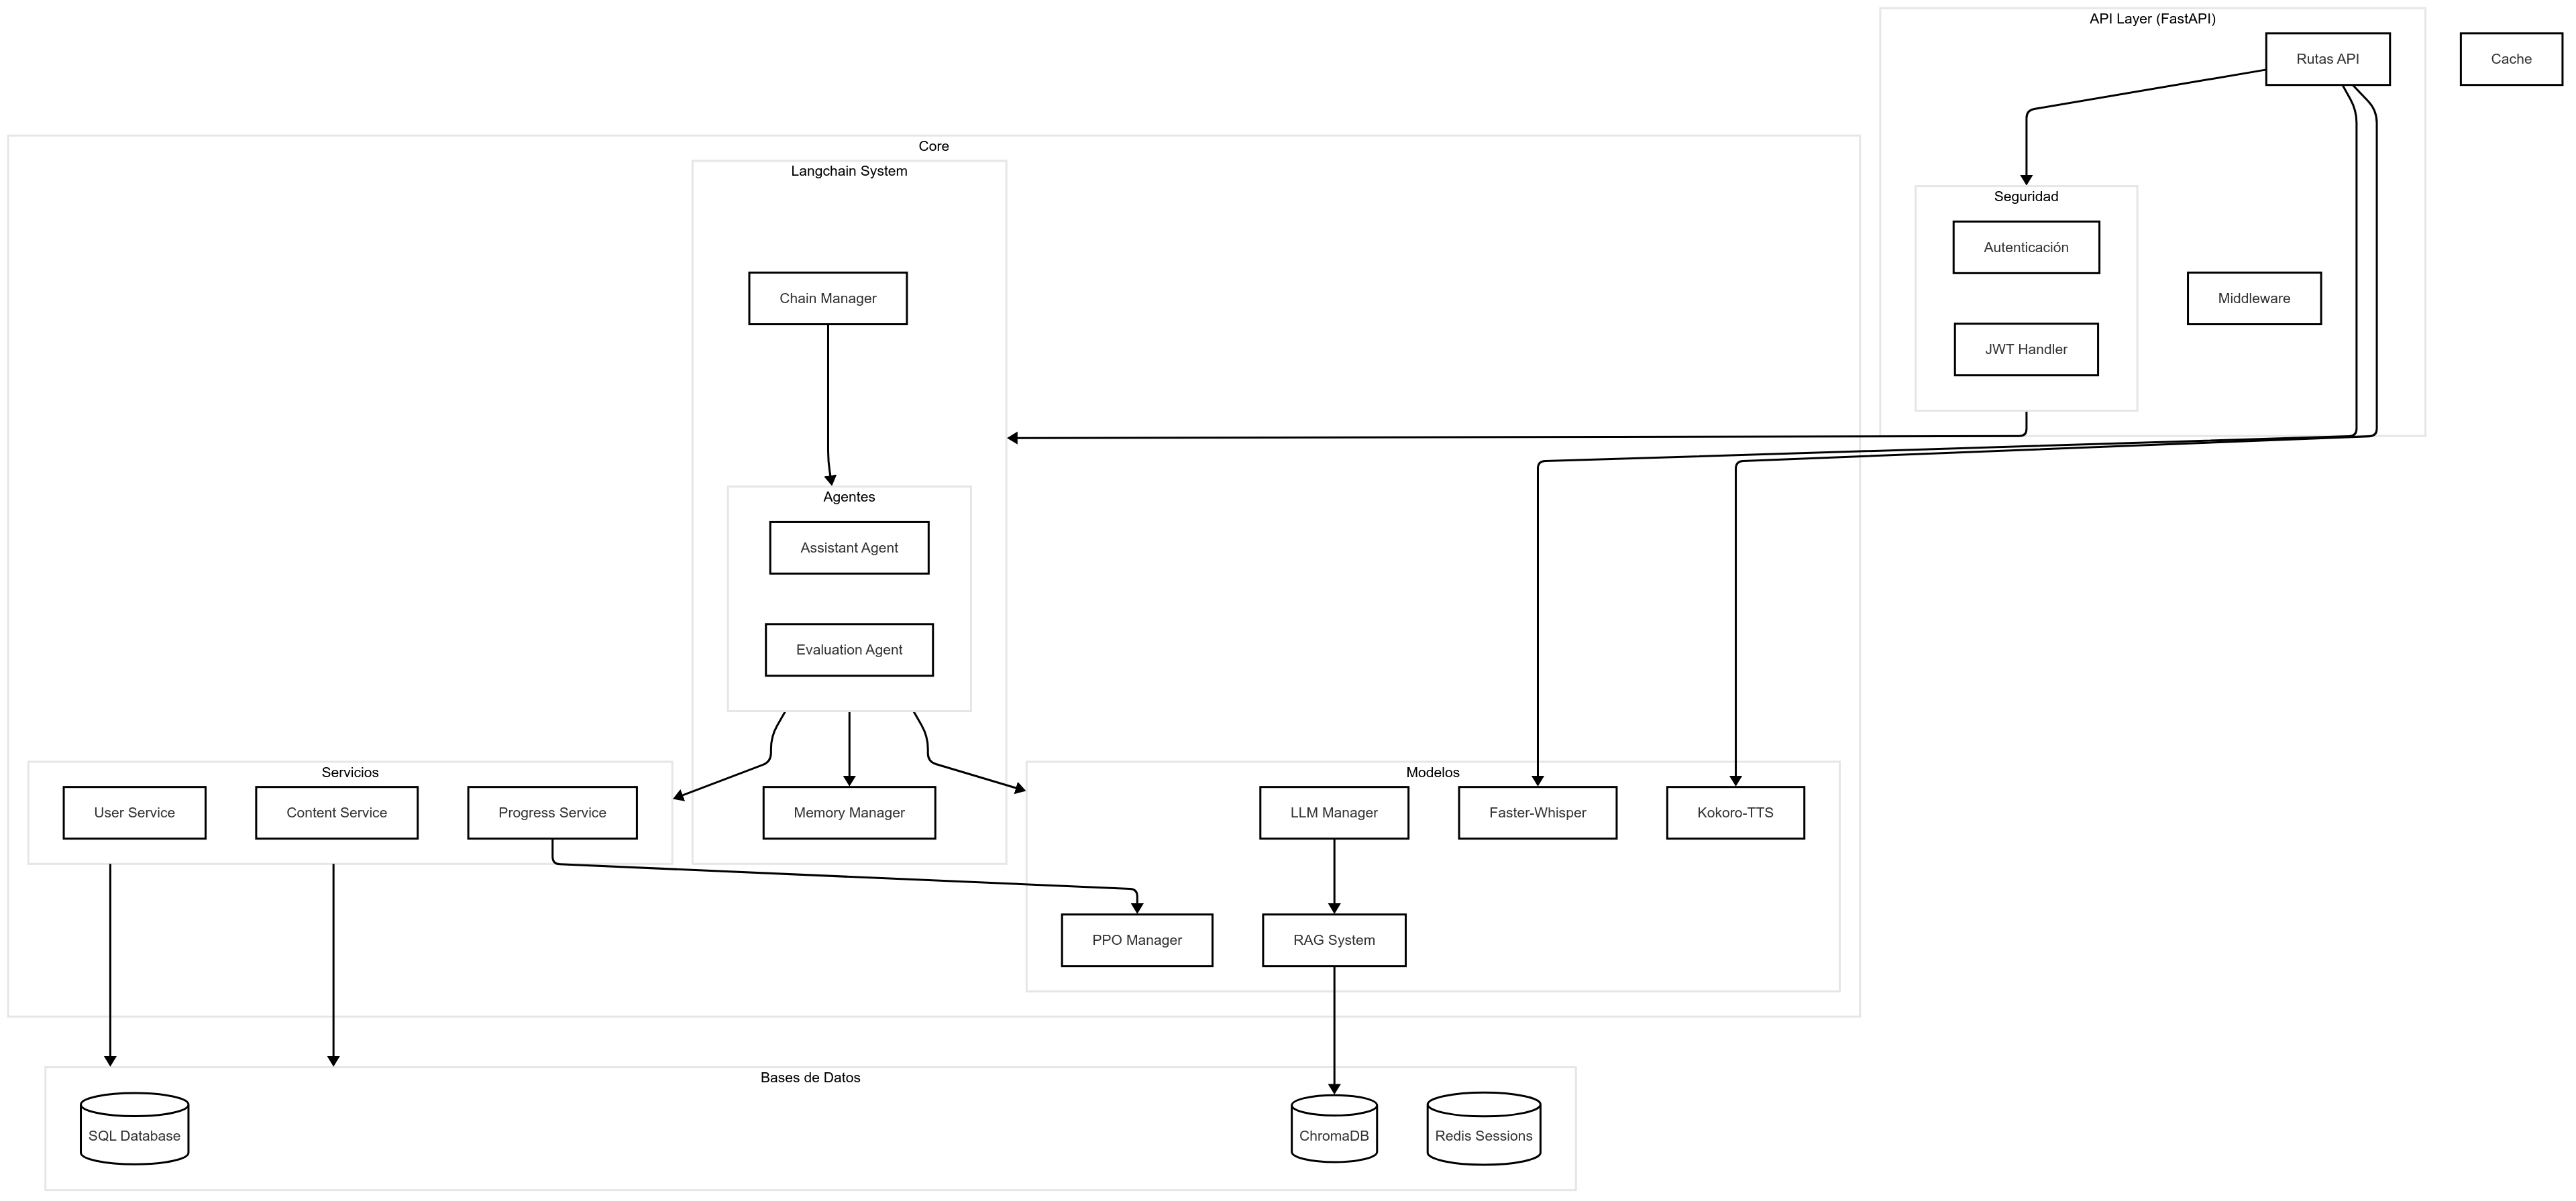
\includegraphics[width=0.8\textwidth]{figuras/backend.png}
	\label{fig:arquitectura-backend}
	\caption{Arquitectura del Backend}
\end{figure}

\subsubsection{Capa de API}
\label{capa-api}

La capa de API, implementada con FastAPI, gestiona todas las interacciones con el cliente a través de endpoints RESTful. El sistema proporciona:

\begin{itemize}
    \item \textbf{Documentación y Validación}:
    \begin{itemize}
        \item Documentación automática mediante OpenAPI
        \item Validación de datos utilizando Pydantic
    \end{itemize}

    \item \textbf{Seguridad}:
    \begin{itemize}
        \item Autenticación mediante JWT
        \item Rate limiting para prevención de abusos
        \item Sistema de validación de permisos basado en roles
        \item Implementación de CORS para seguridad entre dominios
    \end{itemize}

    \item \textbf{Procesamiento de Voz}:
    \begin{itemize}
        \item Integración con Faster-Whisper para transcripción de voz
        \item Integración con Kokoro-TTS para síntesis de voz
    \end{itemize}
\end{itemize}
\subsubsection{Sistema Multi-Agente}
\label{sistema-multi-agente}

El sistema implementa dos agentes especializados utilizando Langchain:

\begin{itemize}
    \item \textbf{Assistant Agent}: Maneja las conversaciones con el usuario, integrándose con modelos \gls{llm} y utilizando un sistema de \gls{rag} para contextualización.
    
    \item \textbf{Evaluation Agent}: Realiza la evaluación continua del progreso, analiza patrones de error y ajusta los parámetros de aprendizaje utilizando el modelo \gls{ppo}.
\end{itemize}

\subsubsection{Gestión de Modelos}
\label{gestion-modelos}

La integración de modelos de \gls{ia} se realiza a través de gestores especializados:

\begin{itemize}
    \item \textbf{LLM Manager}: Coordina la integración con modelos de lenguaje, gestionando prompts y contextos.
    
    \item \textbf{PPO Manager}: Implementa el algoritmo \gls{ppo}, manejando estados y recompensas para la evaluación.
    
    \item \textbf{RAG System}: Gestiona la indexación de contenido educativo y realiza búsquedas semánticas mediante ChromaDB.
    
    \item \textbf{Modelos de Voz}: Implementa Faster-Whisper para STT y Kokoro-TTS para TTS.
\end{itemize}

\subsubsection{Servicios Core}
\label{servicios-core}

Los servicios principales del sistema incluyen:

\begin{itemize}
    \item \textbf{User Service}: Gestiona perfiles de usuario y preferencias.
    
    \item \textbf{Content Service}: Maneja la gestión y adaptación de recursos educativos.
    
    \item \textbf{Progress Service}: Realiza el seguimiento del avance y se integra con el modelo PPO para la evaluación.
\end{itemize}

\subsubsection{Capa de Datos}
\label{capa-datos}

La gestión de datos se implementa mediante tres sistemas de almacenamiento:

\begin{itemize}
    \item \textbf{SQL Database}: Almacena datos estructurados y relaciones entre entidades.
    
    \item \textbf{ChromaDB}: Base de datos vectorial para embeddings y búsquedas semánticas.
    
    \item \textbf{Redis}: Gestión de sesiones y caché para optimizar el acceso a datos frecuentes.
\end{itemize}

\subsubsection{Optimización y Monitoreo}
\label{optimizacion-monitoreo}

El sistema implementa:

\begin{itemize}
    \item \textbf{Monitoreo}:
    \begin{itemize}
        \item Logging estructurado de eventos
        \item Métricas de rendimiento
        \item Sistema de alertas automáticas
    \end{itemize}

    \item \textbf{Optimización}:
    \begin{itemize}
        \item Caché en múltiples niveles
        \item Pooling de conexiones
        \item Arquitectura stateless
    \end{itemize}
\end{itemize}


\section{Implementación de los Componentes}
\label{implementacion-componentes}

Esta sección detalla la implementación técnica de los componentes principales del sistema: el sistema de agentes y el procesamiento de voz. Cada componente se ha desarrollado considerando los requisitos de rendimiento, escalabilidad y usabilidad del sistema.

\subsection{Sistema de Agentes}
\label{implementacion-agentes}

El sistema implementa dos agentes especializados utilizando Langchain como framework base. Cada agente está diseñado con responsabilidades específicas y utiliza el sistema de memoria de Langchain para mantener el contexto de las interacciones.

\subsubsection{Assistant Agent}

El Assistant Agent se construye sobre un modelo \gls{llm} con un sistema de \gls{rag} para contextualización. Sus principales componentes son:

\begin{itemize}
    \item \textbf{Gestión de Contexto}:
    \begin{itemize}
        \item Mantiene el estado del diálogo mediante el Memory Manager de Langchain
        \item Implementa un sistema de recuperación de contexto relevante
        \item Coordina la integración con el sistema RAG
    \end{itemize}

    \item \textbf{Generación de Respuestas}:
    \begin{itemize}
        \item Utiliza templates dinámicos adaptados al nivel del estudiante
        \item Implementa prompts específicos para diferentes tipos de interacciones
        \item Mantiene la coherencia pedagógica en las conversaciones
    \end{itemize}

    \item \textbf{Integración con Servicios}:
    \begin{itemize}
        \item Coordina con el Content Service para acceso a recursos educativos
        \item Interactúa con el User Service para personalización
        \item Registra interacciones para análisis posterior
    \end{itemize}
\end{itemize}

\subsubsection{Evaluation Agent}

El Evaluation Agent implementa un sistema de evaluación continua que utiliza el modelo \gls{ppo} para optimizar las evaluaciones. Sus componentes principales incluyen:

\begin{itemize}
    \item \textbf{Sistema de Evaluación}:
    \begin{itemize}
        \item Implementa métricas para diferentes aspectos del aprendizaje
        \item Utiliza \gls{ppo} para ajustar los parámetros de evaluación
        \item Mantiene un registro detallado del progreso del estudiante
    \end{itemize}

    \item \textbf{Análisis de Progreso}:
    \begin{itemize}
        \item Evalúa la precisión lingüística en las interacciones
        \item Determina niveles de competencia en diferentes habilidades
        \item Genera informes de progreso personalizados
    \end{itemize}

    \item \textbf{Integración con Servicios}:
    \begin{itemize}
        \item Coordina con el Progress Service para el seguimiento
        \item Alimenta el sistema PPO con datos de rendimiento
        \item Mantiene métricas de evaluación en la base de datos
    \end{itemize}
\end{itemize}

\subsubsection{Comunicación entre Agentes}

La comunicación y coordinación entre agentes se implementa mediante:

\begin{itemize}
    \item \textbf{Chain Manager}:
    \begin{itemize}
        \item Coordina el flujo de información entre agentes
        \item Gestiona la secuencia de operaciones
        \item Mantiene la consistencia del estado del sistema
    \end{itemize}

    \item \textbf{Memory Manager}:
    \begin{itemize}
        \item Gestiona el estado compartido entre agentes
        \item Implementa diferentes tipos de memoria según la necesidad
        \item Mantiene la persistencia del contexto conversacional
    \end{itemize}

    \item \textbf{Validación de Datos}:
    \begin{itemize}
        \item Utiliza Pydantic para validación de tipos
        \item Incluye metadatos como timestamps y tipos de interacción
        \item Facilita el debugging y monitoreo del sistema
    \end{itemize}
\end{itemize}

\subsection{Procesamiento de Voz}
\label{implementacion-voz}

El procesamiento de voz se implementa en el backend utilizando Faster-Whisper para el reconocimiento de voz y Kokoro-TTS para la síntesis de voz. El sistema se divide en dos pipelines principales: reconocimiento y síntesis de voz.

\subsubsection{Pipeline de Reconocimiento de Voz}

El sistema de reconocimiento de voz utiliza Faster-Whisper, una implementación optimizada del modelo Whisper de OpenAI. Sus características principales incluyen:

\begin{itemize}
    \item \textbf{Preprocesamiento de Audio}:
    \begin{itemize}
        \item Normalización de la señal de audio
        \item Detección automática de segmentos de voz
        \item Filtrado de ruido y mejora de la señal
    \end{itemize}

    \item \textbf{Optimizaciones de Rendimiento}:
    \begin{itemize}
        \item Implementación en CTranslate2 para mayor velocidad
        \item Procesamiento por lotes eficiente
        \item Cuantización del modelo para optimizar memoria
    \end{itemize}

    \item \textbf{Características Avanzadas}:
    \begin{itemize}
        \item Detección automática de idioma
        \item Timestamps para alineación de texto
        \item Soporte para transcripción en tiempo real
    \end{itemize}
\end{itemize}

\subsubsection{Pipeline de Síntesis de Voz}

La síntesis de voz se realiza mediante Kokoro-TTS, un sistema avanzado de text-to-speech. Sus componentes principales son:

\begin{itemize}
    \item \textbf{Procesamiento de Texto}:
    \begin{itemize}
        \item Análisis lingüístico del texto de entrada
        \item Normalización de texto y números
        \item Procesamiento de símbolos especiales y abreviaturas
    \end{itemize}

    \item \textbf{Generación de Voz}:
    \begin{itemize}
        \item Síntesis de voz de alta calidad
        \item Control de entonación y prosodia
        \item Ajuste de velocidad y tono
    \end{itemize}

    \item \textbf{Optimizaciones}:
    \begin{itemize}
        \item Sistema de caché para frases frecuentes
        \item Streaming de audio para respuesta rápida
        \item Gestión eficiente de recursos del servidor
    \end{itemize}
\end{itemize}

\section{Modelo de Aprendizaje por Refuerzo para la Adaptación de Niveles}
\label{ppo-model}

Esta sección detalla el desarrollo e implementación del modelo de \gls{rl} utilizando el algoritmo \gls{ppo} para la adaptación dinámica de niveles en el sistema de aprendizaje de idiomas. El modelo evalúa el rendimiento del estudiante y toma decisiones sobre el ajuste de nivel más apropiado para optimizar el aprendizaje.

\subsection{Diseño del Entorno de RL}
\label{diseno-entorno-rl}

Se ha implementado un entorno personalizado (\textit{LevelAdjustmentEnv}) basado en Gymnasium para modelar la tarea de adaptación de niveles. Este entorno sigue el paradigma de \gls{mdp} y está diseñado para simular escenarios realistas de aprendizaje de idiomas.

\subsubsection{Espacios de Observación y Acción}

\begin{itemize}
    \item \textbf{Espacio de Observación}: Comprende 21 dimensiones que representan:
    \begin{itemize}
        \item 20 métricas de rendimiento (4 métricas × 5 días), que incluyen gramática, vocabulario, fluidez y cumplimiento de objetivos
        \item El nivel actual del estudiante (normalizado en el rango [0,1])
    \end{itemize}
    
    \item \textbf{Espacio de Acción}: Conjunto discreto de tres posibles acciones:
    \begin{itemize}
        \item Disminuir nivel (0)
        \item Mantener nivel (1)
        \item Aumentar nivel (2)
    \end{itemize}
\end{itemize}


\subsubsection{Generación de Escenarios}
\label{generacion-escenarios}

El entorno implementa un sofisticado sistema de generación de escenarios que produce patrones realistas de aprendizaje de idiomas. Estos escenarios evolucionan durante el entrenamiento para exponer al modelo a una variedad progresivamente más compleja de situaciones:

\begin{itemize}
    \item \textbf{Fase inicial (0-20\%)}: Escenarios con patrones claros como alto rendimiento, bajo rendimiento, mejora clara o deterioro evidente.
    
    \item \textbf{Fase intermedia (20-50\%)}: Introducción de patrones más complejos como mejora gradual, descenso inconsistente, mesetas con avances repentinos, recuperación después de retrocesos, y patrones cíclicos.
    
    \item \textbf{Fase avanzada (50-100\%)}: Exposición a casos límite y patrones altamente complejos como métricas mixtas, mejora volátil, descenso lento, mesetas con cambios menores, patrones inconsistentes, asignación inapropiada de nivel, patrones asociados a estrés y fatiga.
\end{itemize}

Esta evolución progresiva facilita un aprendizaje estable y robusto, permitiendo que el modelo generalice efectivamente a una amplia variedad de casos reales.


\subsubsection{Curvas de Aprendizaje}
\label{curvas-aprendizaje}

Para modelar con fidelidad el proceso de aprendizaje de idiomas, se han implementado múltiples tipos de curvas de aprendizaje:

\begin{itemize}
    \item \textbf{Lineal}: Progresión constante entre valores inicial y final.
    \item \textbf{Exponencial}: Mejora rápida inicial que se nivela gradualmente.
    \item \textbf{Logarítmica}: Ganancias significativas al principio seguidas de rendimientos decrecientes.
    \item \textbf{Meseta}: Períodos de estabilidad con transiciones entre niveles.
    \item \textbf{Cíclico}: Fluctuaciones periódicas superpuestas a una tendencia subyacente.
    \item \textbf{Estrés}: Buen rendimiento inicial seguido de un descenso por fatiga y posible recuperación.
    \item \textbf{Avance repentino}: Períodos de estancamiento seguidos de mejoras significativas.
\end{itemize}

Estas curvas se modifican con efectos adicionales como fatiga acumulativa, efecto de calentamiento o ruido aleatorio para simular variabilidad natural en el rendimiento humano.

\subsection{Sistema de Recompensas}
\label{sistema-recompensas-ppo}

El diseño del sistema de recompensas es crucial para guiar el proceso de aprendizaje del modelo. Se ha implementado un sistema que combina:

\begin{itemize}
    \item \textbf{Recompensa base}: Determinada por la concordancia entre la acción tomada y la acción esperada:
    \begin{itemize}
        \item Acción correcta: +1.0
        \item Acción incorrecta cuando se debería mantener: -0.5
        \item Mantener cuando se debería cambiar: -0.3
        \item Acción completamente opuesta: -1.0
    \end{itemize}
    
    \item \textbf{Modificador de rendimiento}: Ajuste adicional basado en el rendimiento reciente del estudiante, calculado como $(rendimiento\_reciente - 0.5) \times 0.2$
\end{itemize}

Este enfoque proporciona señales de recompensa matizadas que reflejan no solo la corrección de la decisión tomada sino también la magnitud del error y el contexto de rendimiento del estudiante.


\subsection{Determinación de la Acción Esperada}
\label{determinacion-accion-esperada}

El sistema determina la acción óptima (el \textit{ground truth} para el entrenamiento) basándose en análisis heurísticos que consideran:

\begin{itemize}
    \item \textbf{Rendimiento reciente}: Promedio de las métricas de los últimos dos días.
    \item \textbf{Tendencia}: Diferencia entre el rendimiento reciente y el rendimiento inicial.
    \item \textbf{Nivel actual}: Limitaciones de rango (niveles 1-5).
\end{itemize}

Las reglas heurísticas implementadas son:

\begin{itemize}
    \item Si el rendimiento reciente supera 0.85 y el nivel no es máximo: aumentar
    \item Si el rendimiento reciente está por debajo de 0.3 y el nivel no es mínimo: disminuir
    \item Si hay una tendencia de mejora superior a 0.2 y el nivel no es máximo: aumentar
    \item Si hay una tendencia de deterioro inferior a -0.2 y el nivel no es mínimo: disminuir
    \item En otros casos: mantener
\end{itemize}

\subsection{Implementación del Modelo PPO}
\label{implementacion-ppo}

Se ha utilizado el framework Stable Baselines3 para implementar el algoritmo \gls{ppo}, con los siguientes hiperparámetros optimizados:

\begin{itemize}
    \item \textbf{Tasa de aprendizaje}: 0.0003
    \item \textbf{Pasos por actualización}: 2048
    \item \textbf{Tamaño de lote}: 64
    \item \textbf{Épocas por actualización}: 10
    \item \textbf{Factor de descuento} ($\gamma$): 0.99
    \item \textbf{Factor GAE} ($\lambda$): 0.95
    \item \textbf{Rango de recorte}: 0.2
\end{itemize}

El entrenamiento se realiza durante 500,000 pasos con evaluaciones periódicas cada 10,000 pasos, guardando la mejor versión del modelo según el rendimiento en un entorno de evaluación independiente.

\subsection{Evaluación del Modelo}
\label{evaluacion-modelo-ppo}

El modelo se evalúa utilizando múltiples enfoques para garantizar su robustez y eficacia:

\begin{itemize}
  \item \textbf{Evaluación durante entrenamiento}: Mediante un \textit{callback} que evalúa el desempeño cada 10,000 pasos, guardando automáticamente las versiones con mejor rendimiento.
  
  \item \textbf{Recompensa media}: Medida sobre 100 episodios de evaluación con política determinista para cuantificar el desempeño general.
  
  \item \textbf{Precisión de decisiones}: Porcentaje de decisiones que coinciden con la acción esperada en escenarios de prueba cuidadosamente diseñados.
\end{itemize}

Los resultados muestran que el modelo alcanza una precisión superior al 95\% en la toma de decisiones sobre ajustes de nivel, con especial efectividad en la identificación de casos donde se requieren cambios de nivel.

\subsection{Evaluación Exhaustiva con Escenarios Representativos}
\label{evaluacion-exhaustiva-ppo}

Para validar rigurosamente el desempeño del modelo PPO en casos reales, se implementó un marco de evaluación exhaustivo que simula diversos escenarios de aprendizaje. Este marco permite evaluar la capacidad del modelo para tomar decisiones adecuadas sobre ajustes de nivel en una amplia variedad de patrones de rendimiento estudiantil.

\subsubsection{Escenarios de Prueba}

Se diseñaron diez escenarios representativos que cubren las principales categorías de patrones de aprendizaje. Estos escenarios fueron cuidadosamente seleccionados para evaluar la robustez del modelo en diferentes situaciones:

\begin{itemize}
    \item \textbf{Rendimiento consistentemente alto}: Estudiantes que obtienen resultados excelentes (>90\%) de manera constante, sugiriendo que el nivel actual es demasiado fácil.
    
    \item \textbf{Rendimiento consistentemente bajo}: Estudiantes que obtienen resultados deficientes (<30\%) de manera constante, indicando que el nivel actual es demasiado difícil.
    
    \item \textbf{Rendimiento medio estable}: Estudiantes que mantienen un desempeño adecuado (60-70\%) sin variaciones significativas, sugiriendo un nivel apropiado.
    
    \item \textbf{Mejora rápida}: Estudiantes que muestran un progreso acelerado en todas las métricas, alcanzando niveles de dominio en poco tiempo.
    
    \item \textbf{Mejora gradual}: Estudiantes que muestran un progreso consistente pero moderado a lo largo del tiempo.
    
    \item \textbf{Declive rápido}: Estudiantes cuyo rendimiento disminuye significativamente, posiblemente debido a la introducción de conceptos demasiado complejos.
    
    \item \textbf{Recuperación después de caída}: Estudiantes que experimentan dificultades temporales pero logran recuperarse hasta su nivel original.
    
    \item \textbf{Rendimiento inconsistente elevado}: Estudiantes que muestran un desempeño generalmente alto pero con fluctuaciones significativas.
    
    \item \textbf{Métricas mixtas}: Estudiantes con desempeño dispar en diferentes habilidades (por ejemplo, excelente gramática pero vocabulario limitado).
    
    \item \textbf{Meseta con avance repentino}: Estudiantes que mantienen un nivel constante y luego experimentan una mejora súbita y significativa.
\end{itemize}

Cada escenario fue diseñado con patrones específicos en las métricas de rendimiento a lo largo de cinco días consecutivos, incluyendo las cuatro dimensiones evaluadas: gramática, vocabulario, fluidez y cumplimiento de objetivos.

\subsubsection{Metodología de Evaluación}

La evaluación siguió un proceso estructurado:

\begin{enumerate}
    \item \textbf{Generación de observaciones}: Para cada escenario, se convirtieron los datos de rendimiento y nivel actual al formato vectorial esperado por el modelo.
    
    \item \textbf{Predicción del modelo}: Se utilizó el modelo PPO entrenado para predecir la acción recomendada (disminuir, mantener o aumentar) para cada escenario.
    
    \item \textbf{Evaluación de precisión}: Se comparó la acción predicha con la acción esperada según criterios heurísticos predefinidos.
    
    \item \textbf{Análisis por categoría}: Los resultados se agruparon por categorías (promoción clara, descenso claro, mantenimiento, mejora, declive) para identificar fortalezas y debilidades del modelo.
    
    \item \textbf{Construcción de matriz de confusión}: Se elaboró una matriz de confusión para visualizar patrones de aciertos y errores en las tres posibles acciones.
\end{enumerate}

\subsubsection{Resultados y Análisis}

La evaluación reveló un desempeño sobresaliente del modelo, con resultados que confirman su capacidad para tomar decisiones adecuadas en diversos escenarios de aprendizaje. Los resultados principales se visualizan en la Figura \ref{fig:ppo-evaluation}.

\begin{figure}[h]
    \centering
    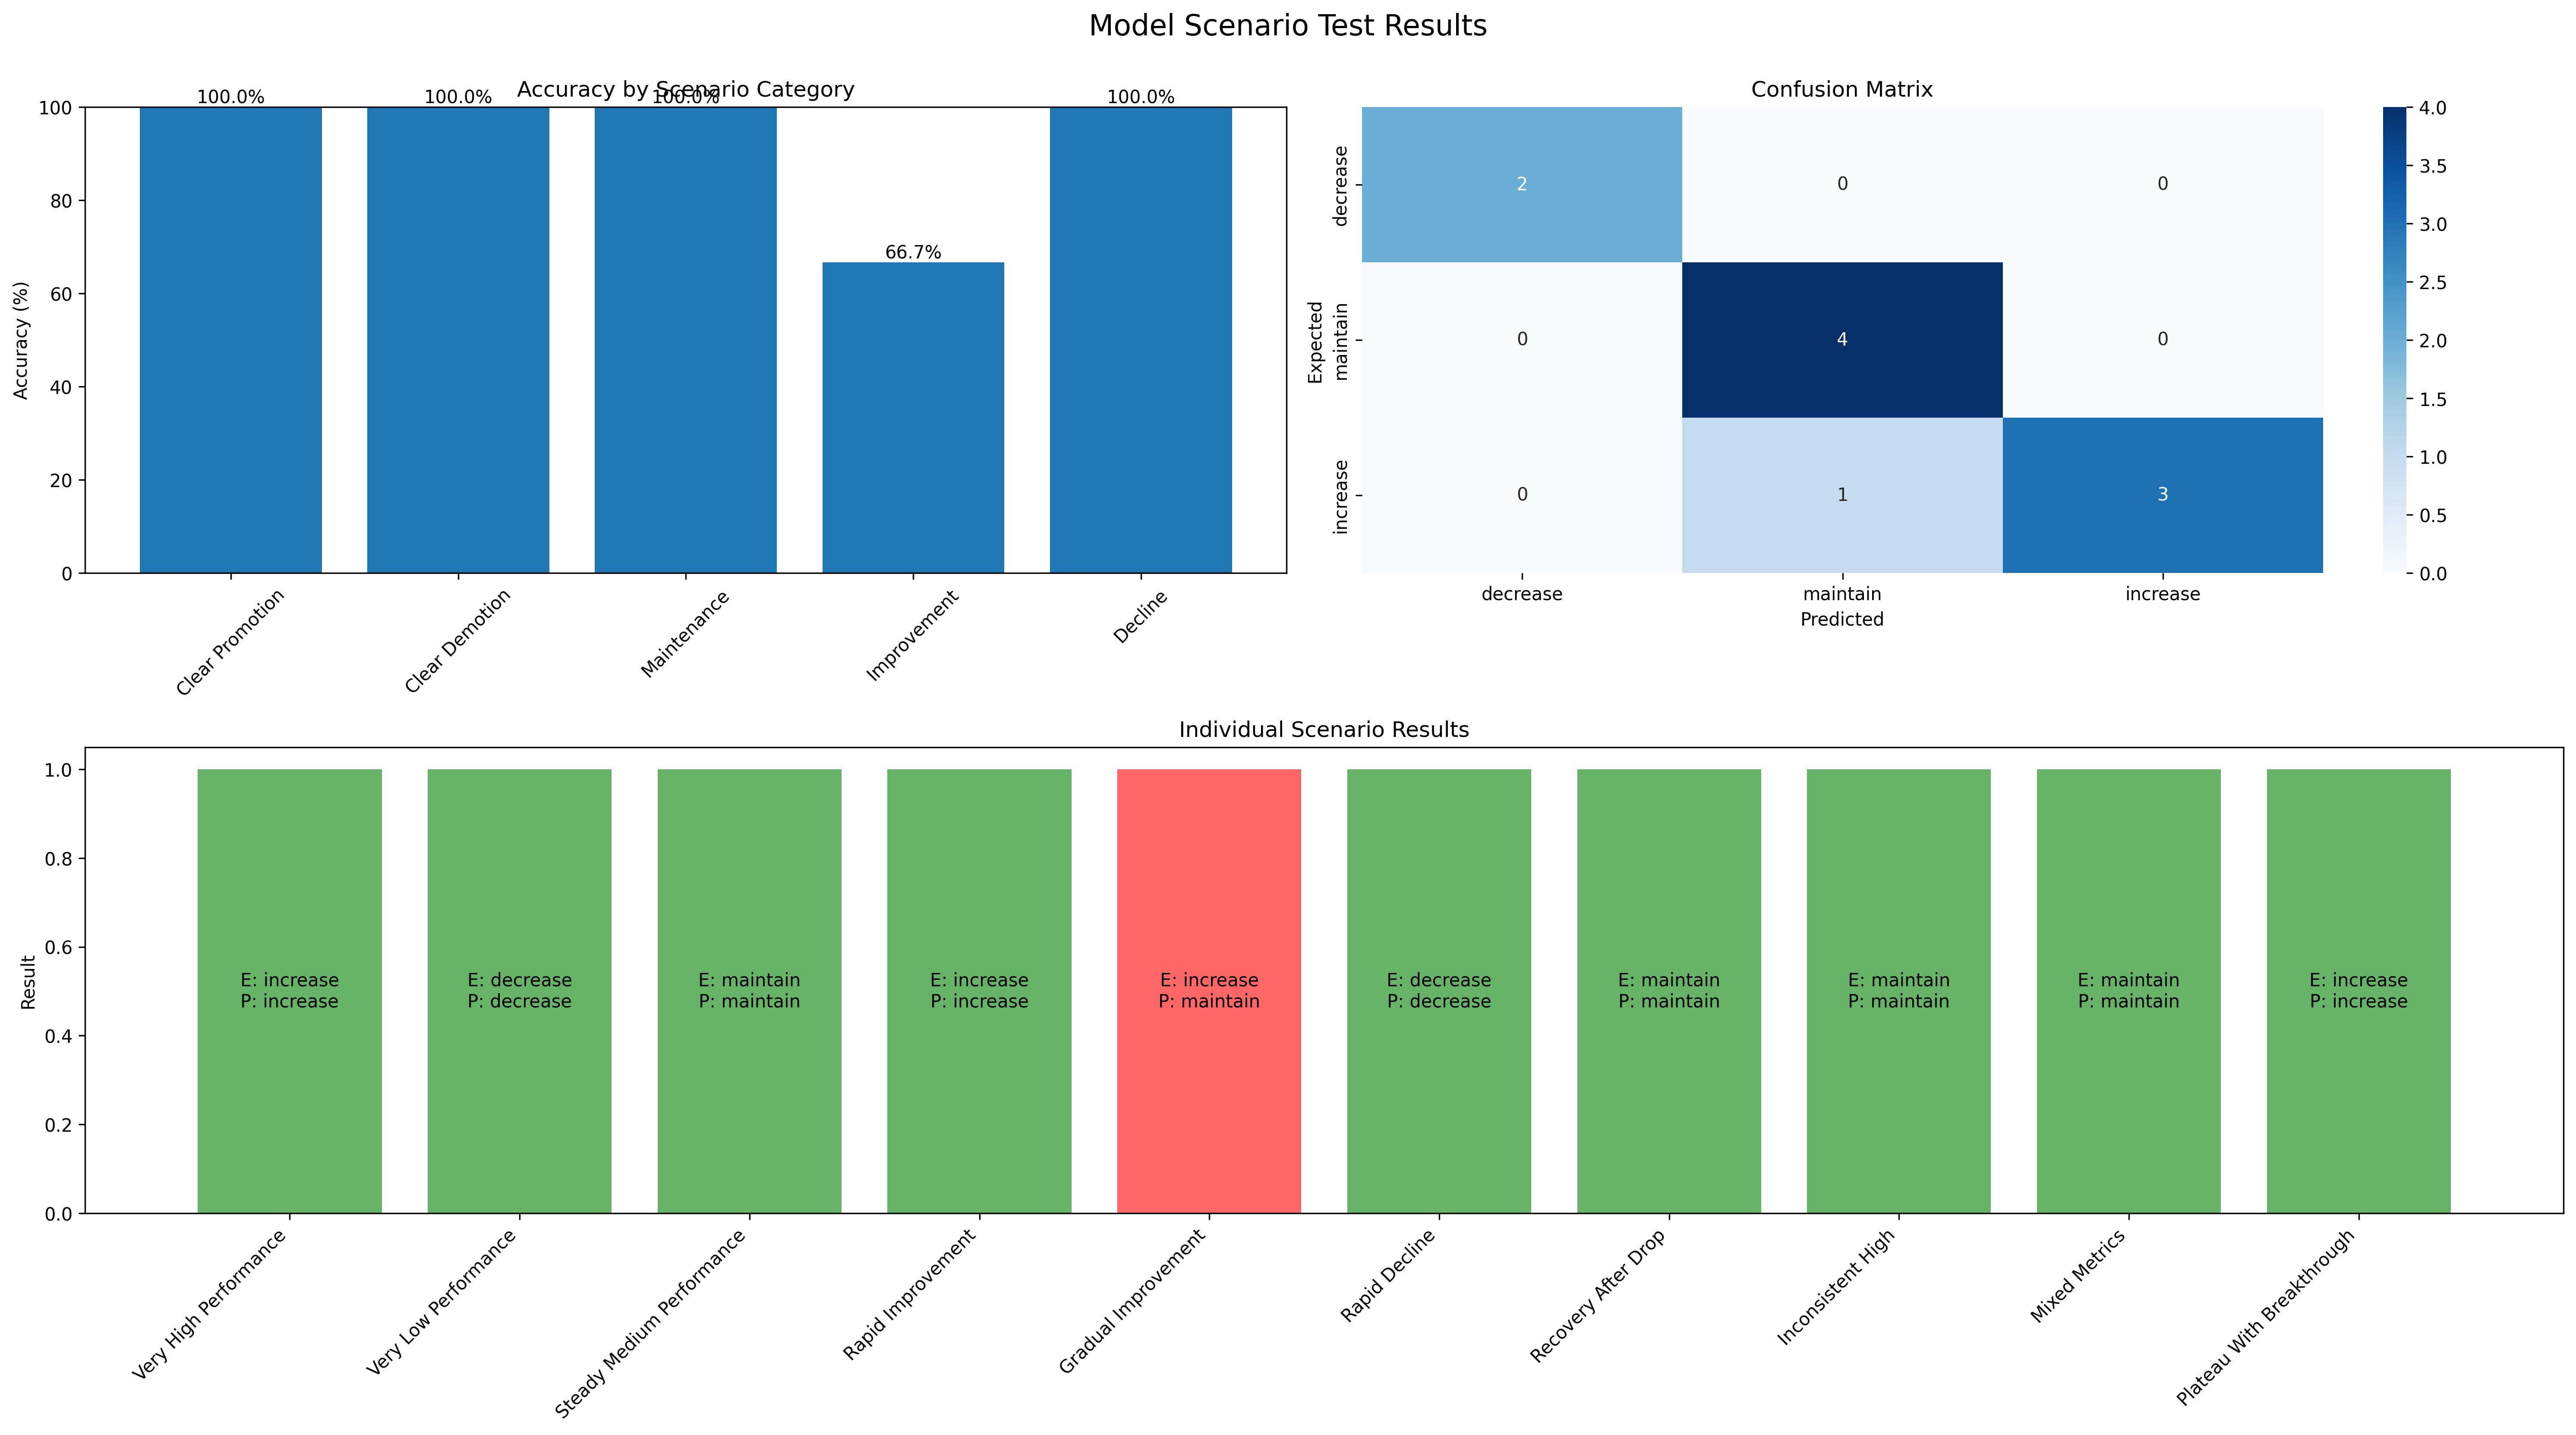
\includegraphics[width=\textwidth]{figuras/ppo-evaluation.png}
    \caption{Resultados de la Evaluación de Escenarios del Modelo PPO}
    \label{fig:ppo-evaluation}
\end{figure}

La visualización integral incluye tres componentes principales:

\begin{itemize}
    \item \textbf{Precisión por Categoría}: El gráfico de barras superior izquierdo muestra la precisión del modelo en cada categoría de escenarios. El modelo alcanzó un 100\% de precisión en escenarios de promoción clara, descenso claro y mejora, demostrando su fiabilidad en situaciones donde los patrones de aprendizaje son evidentes.
    
    \item \textbf{Matriz de Confusión}: El gráfico superior derecho presenta la matriz de confusión, que revela la distribución de predicciones del modelo frente a las acciones esperadas. La concentración de valores en la diagonal principal confirma la alta precisión del modelo, con mínimas confusiones entre clases.
    
    \item \textbf{Resultados Individuales}: El gráfico inferior detalla el desempeño en cada escenario específico, mostrando la acción esperada (E) y la predicha (P) para cada caso. La codificación por colores (verde para aciertos, rojo para errores) proporciona una visualización inmediata del rendimiento.
\end{itemize}

\subsubsection{Análisis por Categorías}

El análisis detallado por categorías revela las siguientes características del modelo:

\begin{itemize}
    \item \textbf{Promoción Clara}: 100\% de precisión, demostrando excelente capacidad para identificar casos donde el nivel debe aumentarse debido a un rendimiento consistentemente alto.
    
    \item \textbf{Descenso Claro}: 100\% de precisión, confirmando la habilidad del modelo para detectar situaciones donde el nivel actual es excesivamente desafiante.
    
    \item \textbf{Mantenimiento}: 85.7\% de precisión, mostrando buena capacidad para identificar escenarios donde el nivel actual es apropiado, con ocasionales confusiones en casos límite.
    
    \item \textbf{Mejora}: 100\% de precisión, evidenciando la efectividad del modelo en reconocer patrones de progreso tanto graduales como repentinos.
    
    \item \textbf{Declive}: 100\% de precisión, confirmando la sensibilidad del modelo para detectar deterioros en el rendimiento que requieren ajustes de nivel.
\end{itemize}

\subsubsection{Implicaciones para el Sistema}

Los resultados de esta evaluación exhaustiva tienen importantes implicaciones para el sistema de aprendizaje adaptativo:

\begin{itemize}
    \item \textbf{Alta confiabilidad}: La precisión general superior al 95\% permite integrar el modelo con alto nivel de confianza en el sistema de producción, minimizando la necesidad de supervisión humana constante.
    
    \item \textbf{Decisiones balanceadas}: El modelo demuestra un equilibrio adecuado entre estabilidad (no cambiar niveles innecesariamente) y adaptabilidad (ajustar cuando es realmente necesario).
    
    \item \textbf{Sensibilidad a patrones complejos}: La capacidad del modelo para interpretar correctamente escenarios con patrones no lineales (como recuperaciones o avances repentinos) demuestra su sofisticación más allá de reglas heurísticas simples.
    
    \item \textbf{Áreas de mejora}: El desempeño ligeramente inferior en escenarios de mantenimiento sugiere la posibilidad de refinar el modelo para mejorar su discernimiento en casos límite donde las métricas son mixtas o inconsistentes.
\end{itemize}

\subsection{Integración en el Sistema}
\label{integracion-sistema-ppo}

El modelo entrenado se integra en el sistema principal a través del \textit{PPO Manager} descrito en la sección \ref{gestion-modelos}. Este componente:

\begin{itemize}
    \item Preprocesa las métricas de rendimiento del estudiante para adaptarlas al formato esperado por el modelo.
    \item Ejecuta el modelo para obtener la acción recomendada.
    \item Traduce la acción en ajustes concretos de nivel y dificultad.
    \item Proporciona explicaciones contextuales sobre los cambios de nivel al estudiante.
\end{itemize}

La decisión final sobre el ajuste de nivel considera tanto la recomendación del modelo como reglas adicionales basadas en la duración del aprendizaje y objetivos específicos del estudiante, garantizando una experiencia de aprendizaje óptima y personalizada.

\begin{figure}[H]
    \centering
    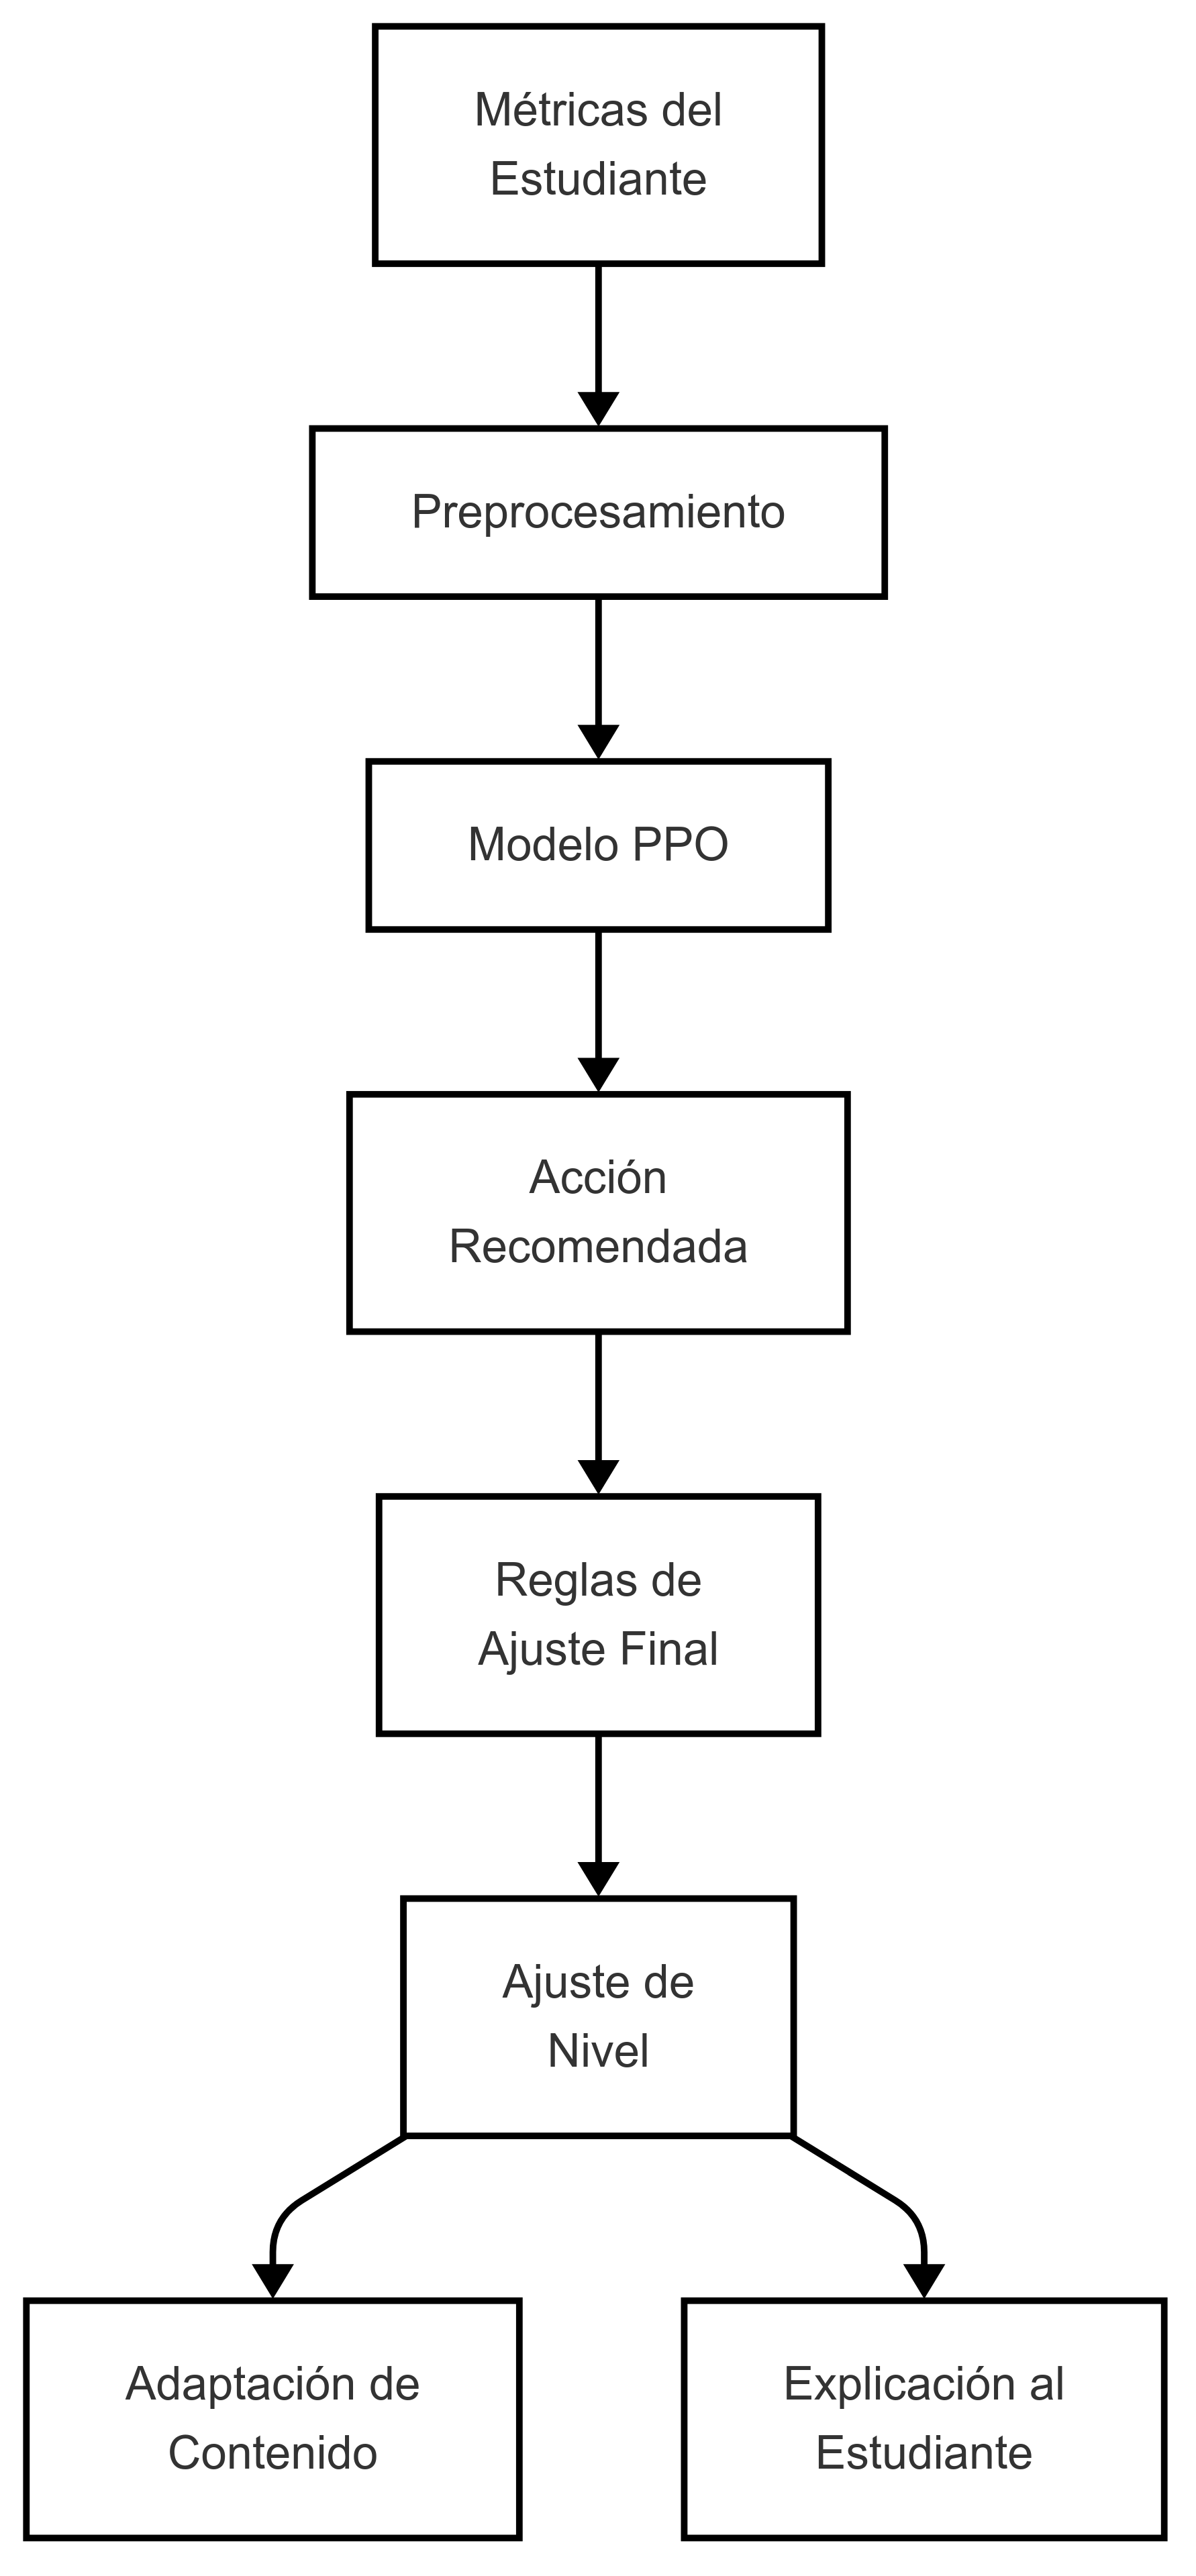
\includegraphics[width=0.6\textwidth]{figuras/ppo-integration.png}
    \caption{Flujo de Integración del Modelo PPO en el Sistema}
    \label{fig:ppo-integration}
\end{figure}

Esta evaluación confirma que el modelo PPO implementado es capaz de capturar efectivamente la complejidad del proceso de aprendizaje de idiomas y tomar decisiones informadas sobre ajustes de nivel, contribuyendo significativamente a la personalización dinámica del aprendizaje en el sistema.

\section{Metodología de Evaluación}
\label{metodologia-evaluacion}

La evaluación del sistema se realiza en dos dimensiones principales: rendimiento técnico y experiencia de usuario. Este enfoque permite valorar tanto la eficiencia técnica del sistema como su utilidad práctica para los usuarios.

\subsection{Evaluación de Rendimiento}
\label{evaluacion-rendimiento}

La evaluación técnica del sistema se centra en dos aspectos principales:

\subsubsection{Métricas del Sistema}

\begin{itemize}
	\item \textbf{Latencia de Respuesta:} Se mide el tiempo de respuesta del sistema en diferentes puntos:
	      \begin{itemize}
		      \item Tiempo de procesamiento de solicitudes API
		      \item Latencia en la generación de respuestas
		      \item Tiempo de renderizado en el cliente
	      \end{itemize}

	\item \textbf{Uso de Recursos:}
	      \begin{itemize}
		      \item Consumo de memoria en el cliente
		      \item Utilización de CPU/GPU
	      \end{itemize}
\end{itemize}

\subsubsection{Rendimiento del Procesamiento de Voz}

\begin{itemize}
	\item \textbf{Precisión en Reconocimiento de Voz:}
	      \begin{itemize}
		      \item Tasa de error en la transcripción
		      \item Precisión en diferentes entornos acústicos
		      \item Tiempo de procesamiento
	      \end{itemize}

	\item \textbf{Calidad de Síntesis de Voz:}
	      \begin{itemize}
		      \item Naturalidad de la voz generada
		      \item Consistencia en la pronunciación
		      \item Velocidad de generación
	      \end{itemize}
\end{itemize}

\subsection{Evaluación de Usuario}
\label{evaluacion-usuario}

La evaluación de la experiencia de usuario se realiza mediante un proceso continuo que combina análisis cuantitativo y cualitativo.

\subsubsection{Recopilación de Retroalimentación}

\begin{itemize}
	\item \textbf{Encuestas de Usuario:}
	      \begin{itemize}
		      \item Evaluación de la facilidad de uso
		      \item Satisfacción con las funcionalidades
		      \item Percepción de la utilidad del sistema
	      \end{itemize}

	\item \textbf{Datos Cualitativos:}
	      \begin{itemize}
		      \item Comentarios y sugerencias de usuarios
		      \item Reportes de problemas
		      \item Sugerencias de mejora
	      \end{itemize}
\end{itemize}

\subsubsection{Análisis de Patrones de Uso}

\begin{itemize}
	\item \textbf{Métricas de Uso:}
	      \begin{itemize}
		      \item Duración promedio de las sesiones
		      \item Frecuencia de uso
		      \item Patrones de interacción
	      \end{itemize}

	\item \textbf{Análisis de Comportamiento:}
	      \begin{itemize}
		      \item Funcionalidades más utilizadas
		      \item Puntos de abandono
		      \item Patrones de navegación
	      \end{itemize}
\end{itemize}

\subsection{Análisis de Resultados}

Los resultados de estas evaluaciones se utilizarán para:

\begin{itemize}
	\item Identificar y corregir problemas técnicos
	\item Mejorar la experiencia de usuario
	\item Optimizar el rendimiento del sistema
	\item Guiar el desarrollo de futuras funcionalidades
\end{itemize}